\section{基于树与规则的分类}
\label{sec:classification-trees}

沿用第\ref{sec:classic-overview-tree-rules}节的条件分支，分类树在叶节点输出类别或类别比例。以下比较分类任务怎样选择分裂、控制生长并确定叶输出；原始结构之外的规则学习则放在同一节中，便于对照条件共享、覆盖与冲突处理。

沿用训练集$D_n=\{(\bm{x}_i,y_i)\}_{i=1}^n$，其中输入有$d$个特征，$y_i\in\{1,\ldots,C\}$。本节允许特征是数值型或类别型，用$D\subseteq D_n$表示到达某个节点的训练样本。建树需要同时确定测试特征、阈值或取值分组，以及叶节点的输出，并非只估计一组预先固定的数值参数。常见做法是在当前节点选择一个能改善类别划分的测试，再递归处理各个子集；为避免把偶然差异也变成分支，还要限制生长或在生长后\term{剪枝}（pruning），即删除缺少预测收益的子树。

图~\ref{fig:classification-tree-partition}把同一个分类器分别画成区域和条件树。在$[0,1]^2$内，$x_1\leq0.5$的输入直接判为类1；其余输入继续检查$x_2$，不超过$0.55$时判为类2，否则判为类1。左图的水平分界只出现在右半区域，正对应右图中第二次测试只对第一个条件不成立的输入执行。这说明树中的路径不仅记录有哪些条件，也规定条件在哪个区域生效。

\begin{figure}[htbp]
  \centering
  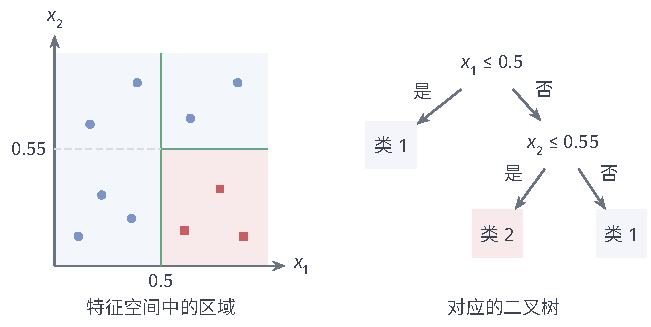
\includegraphics[width=\linewidth]{figures/03-models/01-classic-models/tikz/classification-tree-partition/figure.pdf}
  \caption{二维分类的教学构造。左图为归一化特征空间$[0,1]^2$中的区域划分，圆点表示类1，方点表示类2；右图为产生同一划分的条件树。根节点检查$x_1\leq0.5$，仅在其“否”分支上继续检查$x_2\leq0.55$。点的位置与分裂阈值均为人为设定，不代表真实数据实验。}
  \label{fig:classification-tree-partition}
\end{figure}

不同树算法的主要差异落在三个问题上：怎样评价一次分裂，允许什么样的分支结构，怎样控制树的大小。ID3提供了信息增益驱动的基本构造，C4.5扩展其评分和数据处理方式；CART则采用统一的二叉划分与子树选择框架，形成了另一条决策树研究路线。

\subsection{ID3}
\label{sec:classification-id3}

要决定先检查哪个特征，需要比较“检查前还分不清多少类别”和“检查后还分不清多少类别”。ID3（Iterative Dichotomiser 3）据此选择特征，再在各分支上重复同一过程。Quinlan在1986年的论文中将ID3追溯到Hunt等人的概念学习系统（Concept Learning System, CLS）：CLS向前考察若干层候选树，按测量与误分类代价选择测试；ID3则改用信息驱动的局部评价。这一变化把建树中的“先测什么”落实为当前节点上可计算的信息增益比较，并不保证整棵树最优。本节采用以离散特征、信息增益和不作后剪枝为设定的基本ID3\scite{quinlan1986trees}

\subsubsection{模型结构}
\label{sec:classification-id3-structure}

在节点样本集$D$上，记$p_c(D)$为类别$c$的样本比例。\term{熵}（entropy）用一个数概括类别分布的不确定性：节点只含一类时为零，各类越均匀，熵越大。采用以2为底的对数，
\begin{equation}
  H(D)=-\sum_{c=1}^{C}p_c(D)\log_2 p_c(D),
  \label{eq:classification-entropy}
\end{equation}
其中约定$0\log_2 0=0$。对第$j$个离散特征，令$V_j$为其可能取值集合，$D_{j,v}=\{(\bm{x}_i,y_i)\in D:x_{i,j}=v\}$。该特征的\term{信息增益}（information gain）是分裂前后熵的减少量：
\begin{equation}
  \operatorname{Gain}(D,j)
  =H(D)-\sum_{v\in V_j}\frac{|D_{j,v}|}{|D|}H(D_{j,v}).
  \label{eq:classification-information-gain}
\end{equation}
空子集对求和的贡献定义为零。这里必须按子集大小加权，否则只有一个样本的小分支会与包含大部分样本的分支同样重要。

ID3用选中的特征建立一个内部节点，每个取值对应一个分支。叶节点保存到达该处的类别计数，并通常输出多数类；类别计数相同时使用预先固定的平局规则。这样得到的是分段常值分类器：同一叶区域内的所有输入具有相同预测。叶节点也可报告类别频率，但少量样本上的频率不应被直接理解为可靠的概率估计。

\subsubsection{参数学习}
\label{sec:classification-id3-learning}

从根节点的$D_n$出发，算法计算所有可用特征的信息增益，选择最大者，再分别对其子集递归建树。离散特征已经按取值完全展开后，同一路径上不必再次使用它。若当前样本全部同类，就生成该类叶节点；若可用特征耗尽而标签仍不一致，就输出当前多数类。对训练时未出现的分支，可以保留以父节点多数类为输出的回退叶节点，使预测规则对新输入仍有定义。

每次选择只依据当前节点，因而这是\term{贪心搜索}（greedy search）：接受眼前收益最大的分裂，不回头枚举所有可能的整棵树。基本ID3不在建树后再作剪枝；限制最大深度、最小叶样本数或最小增益，属于另外加入的生长控制。尤其是“增益为零就停止”也会改变基本搜索行为：在异或关系中，单个特征的增益可能为零，而连续两次测试可以完全分开类别。停止规则既能减少无效分裂，也可能阻止发现特征交互。

\subsubsection{小结}
\label{sec:classification-id3-summary}

信息增益把分裂选择变成了可计算的局部比较，却有\term{多值偏差}（multivalued attribute bias）：取值很多的特征更容易把训练样本分成纯净的小组。若每条记录的编号都不同，用编号分裂会使所有子节点熵为零，增益达到$H(D)$，但对一个新编号几乎没有帮助。再加上基本ID3缺少后剪枝，训练集中的噪声也可能变成专门的叶节点。

ID3因此适合说明树怎样从样本中长出来，却不能仅凭训练误差小就获得泛化保证。接下来的C4.5分别处理评分偏差、输入类型和树的规模，保留的仍是这种递归划分思想。

\subsection{C4.5}
\label{sec:classification-c45}

让决策树用于含连续数值和缺失字段的数据，除了换一个分裂分数，还需要约定阈值怎样选择、未知值怎样传递、哪些枝条应当删除。Quinlan在1993年的专著中给出了C4.5的完整程序体系。它沿用ID3的递归构造，同时加入增益率、连续特征测试、缺失值处理、错误估计剪枝和规则提取\scite{quinlan1993c45}

\subsubsection{模型结构}
\label{sec:classification-c45-structure}

多值特征容易得到大增益，是因为它本身就把数据切得很细。C4.5用\term{信息增益率}（gain ratio）比较“类别信息的增加”与“产生这些分支所需的划分信息”。设测试$a$把$D$分成$D_1,\ldots,D_b$，令$q_v=|D_v|/|D|$，则
\begin{align}
  \operatorname{SplitInfo}(D,a)
  &=-\sum_{v=1}^{b}q_v\log_2 q_v,
  \label{eq:classification-split-information}\\
  \operatorname{GainRatio}(D,a)
  &=\frac{\operatorname{Gain}(D,a)}
  {\operatorname{SplitInfo}(D,a)}.
  \label{eq:classification-gain-ratio}
\end{align}
这里的信息增益仍按式\eqref{eq:classification-information-gain}计算，只把按特征取值划分替换为测试$a$的各个结果。分母为零意味着没有真正划分，不能参与比值比较。

归一化并未消除所有问题。若某个测试只分离出极少数样本，其划分信息也很小，微小的增益可能被除法放大。因此，C4.5不是在所有测试中直接取增益率最大者，而是先计算候选测试的平均信息增益，只在增益不低于该平均值的测试中比较增益率。这个筛选避免纯粹依靠小分母取胜；它是启发式约束，并不保证每次都选中最有泛化价值的特征。

\subsubsection{参数学习}
\label{sec:classification-c45-learning}

离散特征可以按取值作多路分裂；连续特征则使用$x_j\leq t$与$x_j>t$的二路测试。候选阈值来自排序后相邻不同取值之间，且分裂后必须满足最小子节点样本量等限制。连续特征在某次分裂后仍可在后代节点使用，因为同一数值轴上可能需要多个阈值。

C4.5各版本对阈值的评价略有区别。较早版本按增益率选择阈值；Quinlan在1996年的修订中先按信息增益选择连续特征的阈值，再扣除搜索阈值所需的描述长度代价，参与特征之间的增益筛选和增益率比较。若有$q$个候选切分位置，这项逐样本惩罚形如$\log_2 q/|D|$，用来抵消“可试阈值更多”带来的选择优势。算法~\ref{alg:classification-c45}突出这些版本共有的建树骨架，把阈值评价留在候选测试生成步骤中\scite{quinlan1996continuous}

\begin{algorithm}[C4.5的递归生长与后剪枝]
  \label{alg:classification-c45}
  \begin{algorithmic}[1]
    \Require 节点样本$D$，可用特征集合$F$，停止及剪枝设置
    \Ensure 剪枝后的分类树
    \Function{Grow}{$D,F$}
      \If{$D$全部同类，或样本量不足，或$F$为空}
        \State \Return 以$D$中多数类为输出的叶节点
      \EndIf
      \State 生成各特征的有效测试，连续特征同时选择阈值
      \State 计算各测试的增益；缺失值按正文约定处理
      \If{没有有效测试，或最大增益不为正}
        \State \Return 以$D$中多数类为输出的叶节点
      \EndIf
      \State 求候选测试的平均增益$\bar g$
      \State 保留增益不低于$\bar g$且划分信息为正的测试
      \State 选择其中增益率最大的测试$a$，建立节点$T$
      \For{测试$a$的每个结果$v$}
        \State 得到相应的子集$D_v$及子问题的特征集合$F_v$
        \If{$D_v$为空}
          \State 将$D$的多数类叶节点接到分支$v$
        \Else
          \State 将$\Call{Grow}{D_v,F_v}$接到分支$v$
        \EndIf
      \EndFor
      \State \Return $T$
    \EndFunction
    \State $T\gets\Call{Grow}{D,F}$
    \State 自底向上比较子树与简化方案的悲观错误估计
    \State \Return 剪枝后的$T$
  \end{algorithmic}
\end{algorithm}

缺失值不能简单地当作已知测试结果。设测试$a$的已知样本总权重占当前节点的比例为$q_{\mathrm{known}}$。C4.5在这些已知样本上估计类别熵的下降，再乘$q_{\mathrm{known}}$降低证据不足的测试所得收益；划分信息还计入未知部分的比例。选定测试后，把缺失该特征的样本按已知样本进入各分支的比例作分数权重分配。后续熵、类别计数和多数类都相应使用权重。预测时遇到缺失值，也按分支权重综合子树的类别预测，而不是随意选一条路径。

树生长完成后，C4.5采用\term{悲观错误剪枝}（pessimistic error pruning）：训练误差倾向于低估新样本错误，因而以二项错误计数的上置信估计作修正，比较保留子树与折叠成多数类叶节点的估计错误数。若简化方案不更差，就可以删除该子树；完整实现还可考察用某个子树提升替代当前分支。置信设置控制剪枝强度，但这种在自适应建树后使用的错误估计是模型选择启发式，不能直接当作整棵树泛化误差的严格置信保证。

树也可以转成规则：每条根到叶路径的测试构成规则前件，叶类别作为后件，再尝试删除不必要条件并筛选规则。未经简化的路径规则继承树的区域划分；条件删除以后可能产生重叠，因此规则系统还必须规定冲突处理和默认预测。这种转换并非只把树的文字抄成一份无序清单。

\subsubsection{小结}
\label{sec:classification-c45-summary}

C4.5对ID3的扩展相互配合：增益筛选和增益率调整局部测试的比较，阈值及缺失值机制扩大可处理的数据范围，后剪枝和规则简化控制最终结构的复杂度。它适合需要检查预测条件的任务，但实际可读性仍取决于树深、规则数和特征含义。单棵树与支持向量机或提升树谁更准确，需要在相同数据划分和调参预算下比较，不能仅由算法名称决定。

\subsection{CART}
\label{sec:classification-cart}

另一种组织树的方法是把每次测试都限定成二选一，再统一研究大树中应保留哪些子树。\term{分类与回归树}（classification and regression trees, CART）采用这一框架；Breiman、Friedman、Olshen与Stone在1984年的专著中将树的构造、最优剪枝与统计性质放在同一体系中讨论。其中，代价复杂度剪枝把“怎样长出一棵大树”与“最终保留多大的子树”分开：生长阶段比较局部分裂，剪枝阶段形成候选子树序列，再用验证选择规模。因此，CART与ID3的区别不只是换一个不纯度指标，还涉及分支结构与整树选择。这里关注分类树；第\ref{sec:regression-cart}节的回归CART复用递归二分与代价复杂度剪枝，但按响应损失选择分裂并在叶内输出数值，本节则按类别不纯度或误分类代价分裂并输出类别标签或类别比例\scite{breiman1984cart}

\subsubsection{模型结构}
\label{sec:classification-cart-structure}

CART分类树通常用\term{基尼不纯度}（Gini impurity）评价节点中类别的混杂程度：
\begin{equation}
  G(D)=1-\sum_{c=1}^{C}p_c(D)^2.
  \label{eq:classification-gini}
\end{equation}
它也等于从节点经验类别分布独立抽取两个标签时，两者不同的概率。对于产生左右子集$D_{\mathrm{L}}$和$D_{\mathrm{R}}$的测试$a$，比较
\begin{equation}
  \Delta G(D,a)=G(D)
  -\sum_{v\in\{\mathrm{L},\mathrm{R}\}}
  \frac{|D_v|}{|D|}G(D_v).
  \label{eq:classification-gini-decrease}
\end{equation}
基尼与熵都鼓励子节点变纯，但并不总给出相同的排序。基尼省去了对数运算，也不意味着整个训练必然更快，因为阈值搜索和数据访问可能占用更多时间。

对连续特征，二分测试仍是阈值比较；对类别特征，测试可写成$x_j\in S$与$x_j\notin S$，其中$S$是部分取值组成的集合。寻找这个集合本身也是搜索问题，取值很多时不能假定枚举所有分组都很便宜。统一的二叉结构便于遍历和剪枝，但可能用多层测试表达一棵多路树的一次分裂。

\subsubsection{参数学习}
\label{sec:classification-cart-learning}

生长阶段反复选择基尼下降最大的有效二分测试，直到满足生长限制，得到一棵较大的树$T_0$。随后进行\term{代价复杂度剪枝}（cost-complexity pruning）：不再逐个比较局部增益，而是在$T_0$的候选子树中平衡拟合误差和叶节点数。令$L(T)$为树$T$的叶节点集合，$\hat c_\ell$为叶$\ell$的预测类别，定义
\begin{align}
  \widehat R(T)
  &=\frac{1}{n}\sum_{\ell\in L(T)}
    \sum_{(\bm{x}_i,y_i)\in D_\ell}
    \mathbb{1}\{y_i\neq\hat c_\ell\},
  \label{eq:classification-cart-empirical-risk}\\
  J_\alpha(T)&=\widehat R(T)+\alpha|L(T)|,
  \qquad \alpha\geq0.
  \label{eq:classification-cart-cost-complexity}
\end{align}
这里$\widehat R(T)$采用全训练集上的误分类比例，使不同子树的误差具有共同尺度。有些软件把叶不纯度的加权和作为剪枝代价；使用其参数时需要核对具体定义，而不能混用不同尺度的$\alpha$。

剪枝路径可以由\term{最弱环节剪枝}（weakest-link pruning）生成。设内部节点$t$以下的子树为$T_t$，把它折叠成一个叶节点后，该区域对全训练集误差的贡献为$\widehat R(t)$；保留时贡献为$\widehat R(T_t)$。两种方案的代价相等时，
\begin{equation}
  \alpha_t=
  \frac{\widehat R(t)-\widehat R(T_t)}
       {|L(T_t)|-1}.
  \label{eq:classification-weakest-link}
\end{equation}
分子是折叠后增加的训练错误，分母是删去的叶数，因而$\alpha_t$衡量“每少保留一个叶节点要付出多少误差”。剪去最小$\alpha_t$对应的分支，再重新计算，就得到从大树到根叶节点的嵌套序列。若某些分支增加叶数却不降低误分类率，可先在$\alpha=0$时合并；临界值处可能有多个最优子树，按一致的最小子树约定处理平局。

对每个$\alpha$，上述序列包含相应的最优剪枝子树，但最优性仅限于给定$T_0$的子树，不是所有可能决策树。实际需要用验证集或交叉验证选择$\alpha$；交叉验证时，各训练折都应独立生长和剪枝，不能先用全体数据确定结构，再把同一结构放入各验证折评分。

\subsubsection{小结}
\label{sec:classification-cart-summary}

把叶节点多数类换成数值均值，把分类不纯度换成平方误差，就得到平方损失下的回归树构造；不需要另换一种树的表示。随机森林常采用这种二叉树，梯度提升方法也常用回归树拟合更新方向。不过，提升树的分裂目标可能来自所用损失的梯度与曲率，不能一概说成直接运行原始CART分类算法。

CART的经典框架还讨论了\term{替代分裂}（surrogate split），即主测试特征缺失时，寻找能够尽量复现主分裂结果的其他特征测试。类别权重和误分类代价也能改变生长与叶预测。具体软件未必实现全部机制；例如scikit-learn的决策树采用优化的CART框架，但类别特征编码和缺失值行为须以相应版本接口为准。二叉结构方便实现，不会自动消除噪声、类别不平衡或数据漂移带来的困难。
